\documentclass[12pt]{article}

% defining image path
\usepackage{graphicx}
\graphicspath{ {./images/} }

% tables
\usepackage[utf8]{inputenc}
\usepackage[table]{xcolor}

\pagestyle{empty}
\setcounter{secnumdepth}{2}

\topmargin=0cm
\oddsidemargin=0cm
\textheight=22.0cm
\textwidth=16cm
\parindent=0cm
\parskip=0.15cm
\topskip=0truecm
\raggedbottom
\abovedisplayskip=3mm
\belowdisplayskip=3mm
\abovedisplayshortskip=0mm
\belowdisplayshortskip=2mm
\normalbaselineskip=12pt
\normalbaselines


\begin{document}

\vspace*{0.5in}
\centerline{\bf\Large
Requirements for the Kakuro project}

\vspace*{0.5in}
\centerline{\bf\Large Iteration 1 COMP354}

\vspace*{0.5in}
\centerline{\bf\Large Team PK-A}

\vspace*{0.5in}
\centerline{\bf\Large 9 February 2020}

\vspace*{1.5in}
\begin{table}[htbp]
\caption{Team Members}
\begin{center}
\begin{tabular}{|c |c | c|}
\hline
Name & Role & ID Number \\
\hline\hline
Tiffany Ah King & Documenter & 40082976 \\
\hline
Isabelle Charette & Coder & 40008121 \\
\hline
Brian Gamboc-Javiniar & Documenter & 40033124 \\
\hline
Vsevolod Ivanov & Coder & 40004286 \\
\hline
Chang Liu & Documenter & 40056360 \\
\hline
Nolan Mckay & Documenter & 27873557 \\
\hline
Nalveer Moocheet & Coder & 40072605 \\
\hline
Hoang Thuan Pham & Documenter & 40022992 \\
\hline
Audrey-Laure St-Louis & Quality Control & 27558783 \\
\hline
Jia Ming Wei & Organizer & 40078192 \\
\hline
\end{tabular}
\end{center}
\end{table}


\newpage



 \renewcommand*\contentsname{Table of Contents}

 

\tableofcontents


\newpage
\section{Introduction}


Kakuro or Kakkuro  is a kind of logic puzzle similar to a crossword but with numbers. It was developed and created by Canadian Jacob E.Funk,an employee of Dell Magazines in 1966. Like Sudoku, solving a Kakuro puzzle involves exploring different combinations and permutations.\\

The objective of the puzzle is to insert a digit from 1 to 9 inclusive into each white cell such that the sum of the numbers in each entry matches the clue associated with it and that no digit is duplicated in any entry. \\

The purpose of this document  is to depict how to use it, its operation, maintenance, or design of software of the kakuro puzzle. It will also describe its functions, graphical user interfaces, requirements and constraints of the game. The details on how to play will be detailed in the use case, diagram and more details will be available in the upcoming design phase.\\


\subsection{Purpose}

This Software Requirements Document (SRD) describes the specification of the Kakuro puzzle game, which is in partial fulfillment of the requirements of COMP 354- Introduction to Software Engineering. It will define the requirements of the user interfaces, user stories, the rules and how this software works.The analysis model will include use UML, case diagrams, class diagrams, sequence diagrams and state transition diagrams. Furthermore, a detailed
project plan will be provided, including the schedule of the upcoming phases. This document is intended primarily for the members of  Team PK-A and the project co-ordinator, Dr. Gregory Butler, as it will serve as a basis for the upcoming phases of the project.
 

\subsection{Scope}

Screen shots of the user interfaces will give the player an idea on how the game will look once it is completed. The user case will be based on every scenarios possible when the game is being played. The user description will include the target audience and working environment of the game. Specifications for the game will be outlined in the specific requirements section and the analysis model will contain UML diagrams. The use case diagrams will give an overview of the functions of Kakuro and how the users will interact with the game. The class diagrams will show the interrelationships between the different objects in the game and the sequence diagrams will model the flow of logic within the game.



\subsection{Context}

The software we are building is a puzzle game called Kakuro, which we are solely building it as a desktop application. We will be building other features in conjunction with the game mechanics of Kakuro as part of the experience that differs from the usual gameplay. The users are players of the game, who are able to interact with the application by playing as a known or as an anonymous user. The desktop application will utilize a database to store information, such as scores, users, difficulties, and other important information. 


\subsection{Business Goals}

The objective of this project is to design and implement a single-player desktop application of the game Kukuro. The application will enforce the rules of a classical Kukuro game. It will allow a single player to play a random 10x10 Kakuro, and it will also keep track of the best play record of each registered user. 



\section{Domain Model}

\begin{figure}[htbp]
    \centering
    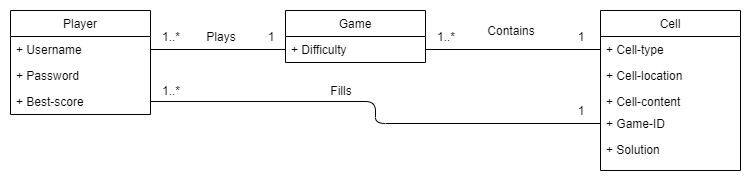
\includegraphics[scale=0.6]{DomainModel}
    \caption{Our current system}
    \label{fig:DomainModel}
\end{figure}


\section{Actors}
Anonymous user \\\\
Anonymous users are players who are not registered but want to play the game without having added value to their gameplay. They have the same functionality as a normal user, but they have limited usage with the software application. If the anonymous user wants to ever save their score into our system, they will need to create an account. (no timer / not able to pause  if we allow timer / not able to view highscores of others /  other things?) \\

Registered user\\\\
Registered users are users who created an account and are able to fully use all the features in the desktop application. As a registered user, they can view the overall scores of all users, as well as their personal scores.\\

%%%%%%%%%%%%%%%%%%%%%%%%%%%%% USE CASE 1 - make a function to not repeat

\section{Use Cases}
\subsubsection{Use Case 1 - Start the game} \label{uc:1}

\begin{figure}[htbp]
    \centering
    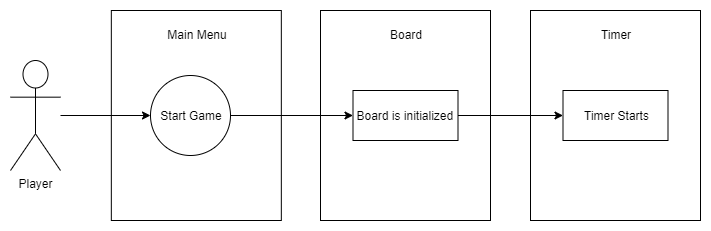
\includegraphics[scale=0.6]{StartGame}
    \caption{Use Case Diagram - Start the game}
    \label{fig:StartGame}
\end{figure}

\begin{center}
\setlength{\tabcolsep}{18pt}
\renewcommand{\arraystretch}{1.3}
\begin{tabular}{ |p{3cm}|p{10cm}| }
    \hline
    \rowcolor{green}
   Item & Description \\
    \hline
    Name & Start the game \\
    \hline
    Summary & A player starts the game \\
    \hline
    Actors & Player \\
    \hline
    Precondition & None \\
    \hline
    Main Scenario &     
    \vspace*{-0.2in}
    \begin{enumerate}
    \item The user starts the game
    \item The board is initialized
    \item Timer starts
    \end{enumerate}  \\
    \hline
    Exceptions &  \\
    \hline
    Postcondition & 
    \vspace*{-0.2in}
    \begin{enumerate}
    \item The player can now input answers
    \end{enumerate}  \\
    \hline
    Priority & High  \\
    \hline
    Traces to Test Cases & Added when test cases done  \\
    \hline
\end{tabular}
\end{center}

\newpage

%%%%%%%%%%%%%%%%%%%%%%%%%%%%% USE CASE 2 - make a function to not repeat

\subsubsection{Use Case 2 - Submit answer} \label{uc:2}

\begin{figure}[htbp]
    \centering
    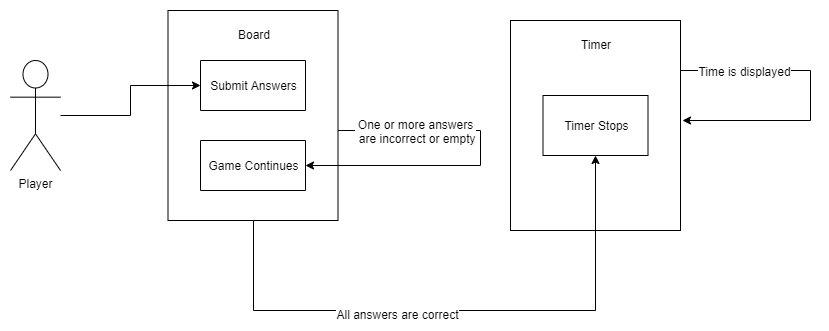
\includegraphics[scale=0.6]{SubmitAnswers}
    \caption{Use Case Diagram - Submit answer}
    \label{fig:SubmitAnswers}
\end{figure}

\begin{center}
\setlength{\tabcolsep}{16pt}
\renewcommand{\arraystretch}{1.1}
\begin{tabular}{ |p{3cm}|p{10cm}| }
    \hline
    \rowcolor{green}
   Item & Description \\
    \hline
    Name & Submit Answer \\
    \hline
    Summary & Player checks if the input is complete \\
    \hline
    Actors & Player \\
    \hline
    Precondition & Game has started \\
    \hline
    Main Scenario &     
    \vspace*{-0.1in}
    \begin{enumerate}
    \item The player submit answers
    \item The answers are correct
    \item Timer stops and time is shown
    \item Game ends
    \item Other paths
        \begin{enumerate}
            \item One or more of the answers are empty or incorrect
            \item Game continues
        \end{enumerate}
    \end{enumerate}  \\
    \hline
    Exceptions &  \\
    \hline
    Postcondition & 
    \vspace*{-0.2in}
    \begin{enumerate}
    \item User keeps playing
    \item Main menu appears
    \end{enumerate}  \\
    \hline
    Priority & High  \\
    \hline
    Traces to Test Cases & Added when test cases done  \\
    \hline
\end{tabular}
\end{center}

\newpage

%%%%%%%%%%%%%%%%%%%%%%%%%%%%% USE CASE 3 - make a function to not repeat

\subsubsection{Use Case 3 - Quit Game} \label{uc:3}

\begin{figure}[htbp]
    \centering
    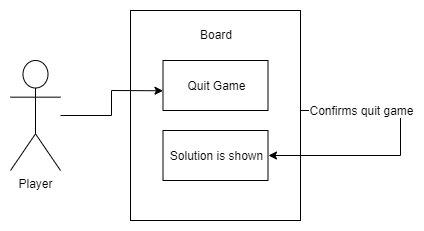
\includegraphics[scale=0.6]{QuitGame}
    \caption{Use Case Diagram - Quit Game}
    \label{fig:QuitGame}
\end{figure}

\begin{center}
\setlength{\tabcolsep}{18pt}
\renewcommand{\arraystretch}{1.3}
\begin{tabular}{ |p{3cm}|p{10cm}| }
    \hline
    \rowcolor{green}
   Item & Description \\
    \hline
    Name & Quit game \\
    \hline
    Summary & The game has started \\
    \hline
    Actors & User \\
    \hline
    Precondition & The game was played \\
    \hline
    Main Scenario &     
    \vspace*{-0.2in}
    \begin{enumerate}
    \item The player selects quit game
    \item Confirmation shown
    \item User confirms exit
    \item The game ended
    \item Solution is shown
    \item Other paths
        \begin{enumerate}
            \item User declines confirmation
            \item Game continues
        \end{enumerate}
    \end{enumerate}  \\
    \hline
    Exceptions &  \\
    \hline
    Postcondition & 
    \vspace*{-0.2in}
    \begin{enumerate}
        \item Main menu appears
    \end{enumerate}  \\
    \hline
    Priority & High  \\
    \hline
    Traces to Test Cases & Added when test cases done  \\
    \hline
\end{tabular}
\end{center}

\newpage

%%%%%%%%%%%%%%%%%%%%%%%%%%%%% USE CASE 4 - make a function to not repeat

\subsubsection{Use Case 4 - Restart Game} \label{uc:4}

\begin{figure}[htbp]
    \centering
    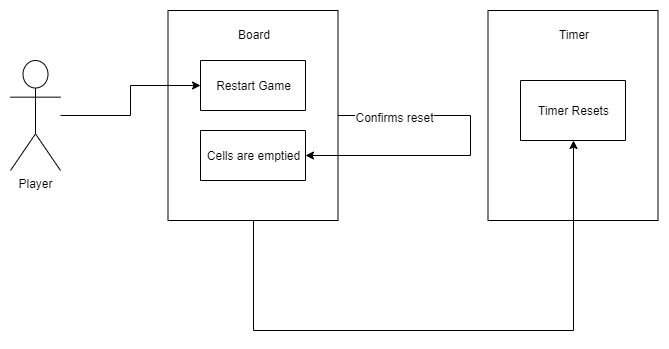
\includegraphics[scale=0.6]{RestartGame}
    \caption{Use Case Diagram - Restart Game}
    \label{fig:RestartGame}
\end{figure}

\begin{center}
\setlength{\tabcolsep}{18pt}
\renewcommand{\arraystretch}{1.3}
\begin{tabular}{ |p{3cm}|p{10cm}| }
    \hline
    \rowcolor{green}
   Item & Description \\
    \hline
    Name & Restart game \\
    \hline
    Summary & The game will be restarted and all the cells be return to empty and the timer will reset \\
    \hline
    Actors & Player \\
    \hline
    Precondition & The game has started \\
    \hline
    Main Scenario &     
    \vspace*{-0.2in}
    \begin{enumerate}
    \item The player selects restart game
    \item Confirmation shown
    \item User confirms
    \item All input is deleted and all cells are empty
    \item Timer resets
    \item Other paths
        \begin{enumerate}
            \item User declines confirmation
            \item Game continues
        \end{enumerate}
    \end{enumerate}  \\
    \hline
    Exceptions &  \\
    \hline
    Postcondition & 
    \vspace*{-0.2in}
    \begin{enumerate}
        \item Game begins
    \end{enumerate}  \\
    \hline
    Priority & High  \\
    \hline
    Traces to Test Cases & Added when test cases done  \\
    \hline
\end{tabular}
\end{center}

\newpage

%%%%%%%%%%%%%%%%%%%%%%%%%%%%% USE CASE 5 - Choose difficulty level

\subsubsection{Use Case 5 - Choose difficulty level} \label{uc:5}

\begin{figure}[htbp]
    \centering
    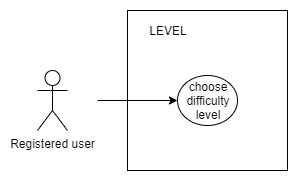
\includegraphics[scale=0.6]{LevelDifficulty}
    \caption{Use Case Diagram - Choose difficulty level}
    \label{fig:LevelDifficulty}
\end{figure}

\begin{center}
\setlength{\tabcolsep}{18pt}
\renewcommand{\arraystretch}{1.3}
\begin{tabular}{ |p{3cm}|p{10cm}| }
    \hline
    \rowcolor{green}
   Item & Description \\
    \hline
    Name & Choose difficulty level \\
    \hline
    Summary & A registered user can choose the level of difficulty from level 1-3 \\
    \hline
    Actors & Registered user \\
    \hline
    Precondition & 
    \vspace*{-0.2in}
    \begin{enumerate}
        \item The user is logged in
        \item The user pressed start game
    \end{enumerate}  \\
    \hline
    Main Scenario &     
    \vspace*{-0.2in}
    \begin{enumerate}
        \item The user views the 'choose a level screen' which displays level 1-3
        \item The user selects the level
        \item The user views the grid and can now start the gameplay
    \end{enumerate}  \\
    \hline
    Exceptions &  \\
    \hline
    Postcondition & 
    \vspace*{-0.2in}
    \begin{enumerate}
        \item Game begins
    \end{enumerate}  \\
    \hline
    Priority & Low  \\
    \hline
    Traces to Test Cases & Added when test cases done  \\
    \hline
\end{tabular}
\end{center}

\newpage

%%%%%%%%%%%%%%%%%%%%%%%%%%%%% USE CASE 6 - Input number

\subsubsection{Use Case 6 - Input number} \label{uc:6}

\begin{figure}[htbp]
    \centering
    % \includegraphics[scale=0.6]{MIA}
    \caption{Use Case Diagram - Input number ----- \textbf{missing}}
    % \label{fig:MIA}
\end{figure}

\begin{center}
\setlength{\tabcolsep}{18pt}
\renewcommand{\arraystretch}{1}
\begin{tabular}{ |p{3cm}|p{10cm}| }
    \hline
    \rowcolor{green}
   Item & Description \\
    \hline
    Name & Input number \\
    \hline
    Summary & The player choose and enter a number from 0-9 into a blank cell \\
    \hline
    Actors & Player \\
    \hline
    Precondition & 
    \vspace*{-0.2in}
    \begin{enumerate}
        \item Game is in progress
    \end{enumerate}  \\
    \hline
    Main Scenario &     
    \vspace*{-0.2in}
    \begin{enumerate}
        \item The player chooses a blank cell
        \item The player enters a number between 0-9
        \item The number chosen by the player is shown in the blank cell
        \item Use case terminates successfully
    \end{enumerate}  \\
    \hline
    Alternate Scenario &     
    \vspace*{-0.2in}
    \begin{enumerate}
        \item The player chooses a blank cell that is already filled
        \item The player enters a number between 0-9
        \item The number previously shown in the cell is removed and the new selected number is shown in the cell
        \item Use case terminates successfully
    \end{enumerate}  \\
    \hline
    Exceptions & 
    \begin{enumerate}
        \item The player enters a letter
        \item The use case terminates unsuccessfully
    \end{enumerate}  \\
    \hline
    Postcondition & 
    \vspace*{-0.2in}
    \begin{enumerate}
        \item The selected number is shown in the selected cell
    \end{enumerate}  \\
    \hline
    Priority & High  \\
    \hline
    Traces to Test Cases & Added when test cases done  \\
    \hline
\end{tabular}
\end{center}

\newpage

%%%%%%%%%%%%%%%%%%%%%%%%%%%%% USE CASE 7 - Pause game

\subsubsection{Use Case 7 - Pause game} \label{uc:7}

\begin{figure}[htbp]
    \centering
    % \includegraphics[scale=0.6]{MIA}
    \caption{Use Case Diagram - Pause game --- \textbf{missing}}
    % \label{fig:MIA}
\end{figure}

\begin{center}
\setlength{\tabcolsep}{18pt}
\renewcommand{\arraystretch}{1.3}
\begin{tabular}{ |p{3cm}|p{10cm}| }
    \hline
    \rowcolor{green}
   Item & Description \\
    \hline
    Name & Pause game \\
    \hline
    Summary & The player pauses the game he/she is currently playing \\
    \hline
    Actors & Player \\
    \hline
    Precondition & 
    \vspace*{-0.2in}
    \begin{enumerate}
        \item There is a game in progress
    \end{enumerate}  \\
    \hline
    Main Scenario &     
    \vspace*{-0.2in}
    \begin{enumerate}
        \item The player clicks on the pause button
        \item The game board becomes black
        \item The application informs the player that the game is paused
        \item Use case terminates successfully
    \end{enumerate}  \\
    \hline
    Exceptions &  \\
    \hline
    Postcondition & \\
    \hline
    Priority & Medium  \\
    \hline
    Traces to Test Cases & Added when test cases done  \\
    \hline
\end{tabular}
\end{center}

\newpage

%%%%%%%%%%%%%%%%%%%%%%%%%%%%% USE CASE 8 - Resume game

\subsubsection{Use Case 8 - Resume game} \label{uc:8}

\begin{figure}[htbp]
    \centering
    % \includegraphics[scale=0.6]{MIA}
    \caption{Use Case Diagram - Resume game --- \textbf{missing}}
    % \label{fig:MIA}
\end{figure}

\begin{center}
\setlength{\tabcolsep}{18pt}
\renewcommand{\arraystretch}{1.3}
\begin{tabular}{ |p{3cm}|p{10cm}| }
    \hline
    \rowcolor{green}
   Item & Description \\
    \hline
    Name & Resume game \\
    \hline
    Summary & The player resumes a game that is currently playing \\
    \hline
    Actors & Player \\
    \hline
    Precondition & 
    \vspace*{-0.2in}
    \begin{enumerate}
        \item There is a game being paused
    \end{enumerate}  \\
    \hline
    Main Scenario &     
    \vspace*{-0.2in}
    \begin{enumerate}
        \item The player clicks on the resume button
        \item The game board is revealed to the user
        \item The timer starts ticking again
        \item Use case terminates successfully
    \end{enumerate}  \\
    \hline
    Exceptions &  \\
    \hline
    Postcondition & \\
    \hline
    Priority & Medium  \\
    \hline
    Traces to Test Cases & Added when test cases done  \\
    \hline
\end{tabular}
\end{center}

\newpage

%%%%%%%%%%%%%%%%%%%%%%%%%%%%% USE CASE 9 - Login

\subsubsection{Use Case 9 - Login} \label{uc:9}

\begin{figure}[htbp]
    \centering
    % \includegraphics[scale=0.6]{MIA}
    \caption{Use Case Diagram - Login --- \textbf{missing}}
    % \label{fig:MIA}
\end{figure}

\begin{center}
\setlength{\tabcolsep}{18pt}
\renewcommand{\arraystretch}{1.3}
\begin{tabular}{ |p{3cm}|p{10cm}| }
    \hline
    \rowcolor{green}
   Item & Description \\
    \hline
    Name & Login \\
    \hline
    Summary & The player signs into his or her game account \\
    \hline
    Actors & Player \\
    \hline
    Precondition & \\
    \hline
    Main Scenario &     
    \vspace*{-0.2in}
    \begin{enumerate}
        \item The player provides a username and a password
        \item The application authenticates the user
        \item The application informs the player that login was successful
        \item Use case terminates successfully
    \end{enumerate}  \\
    \hline
    Exceptions & 
    \vspace*{-0.2in}
    \begin{enumerate}
        \item The player enters an invalid username or password
        \item The application informs the player that login was unsuccessful
        \item Use case terminates unsuccessfully
    \end{enumerate}  \\
    \hline
    Postcondition & \\
    \hline
    Priority & Medium  \\
    \hline
    Traces to Test Cases & Added when test cases done  \\
    \hline
\end{tabular}
\end{center}

\newpage

%%%%%%%%%%%%%%%%%%%%%%%%%%%%% USE CASE 10 - Register player

\subsubsection{Use Case 10 - Register player} \label{uc:10}

\begin{figure}[htbp]
    \centering
    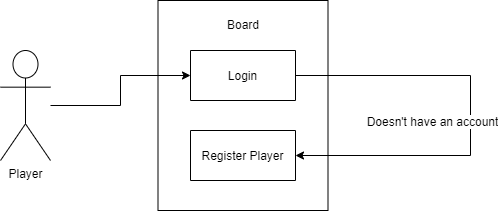
\includegraphics[scale=0.6]{images/RegisterPlayer.png}
    \caption{Use Case Diagram - Register Player}
    \label{fig:RegisterPlayer}
\end{figure}

\begin{center}
\setlength{\tabcolsep}{18pt}
\renewcommand{\arraystretch}{1.3}
\begin{tabular}{ |p{3cm}|p{10cm}| }
    \hline
    \rowcolor{green}
   Item & Description \\
    \hline
    Name & Register player \\
    \hline
    Summary & The user is able to register in order to play the kakuro game \\
    \hline
    Actors & Player \\
    \hline
    Precondition & 
    \vspace*{-0.2in}
    \begin{enumerate}
        \item The user entered the application
        \item The user pressed register button
    \end{enumerate}  \\
    \hline
    Main Scenario &     
    \vspace*{-0.2in}
    \begin{enumerate}
        \item The user clicks the register button
        \item the user registers by inputting username and password
        \item The user gets his own account and starts game
    \end{enumerate}  \\
    \hline
    Exceptions & 
    \vspace*{-0.2in}
    \begin{enumerate}
        \item Username and password are not following the validations
        \item The second password input doesn't match the first one
        \item User name and password are too weak
    \end{enumerate}  \\
    \hline
    Postcondition &
    \vspace*{-0.2in}
    \begin{enumerate}
        \item Login
        \item Game start
    \end{enumerate}  \\
    \hline
    Priority & High \\
    \hline
    Traces to Test Cases & Added when test cases done  \\
    \hline
\end{tabular}
\end{center}

\newpage

%%%%%%%%%%%%%%%%%%%%%%%%%%%%% USE CASE 11 - Save game

\subsubsection{Use Case 11 - Save Game} \label{uc:11}

\begin{figure}[htbp]
    \centering
    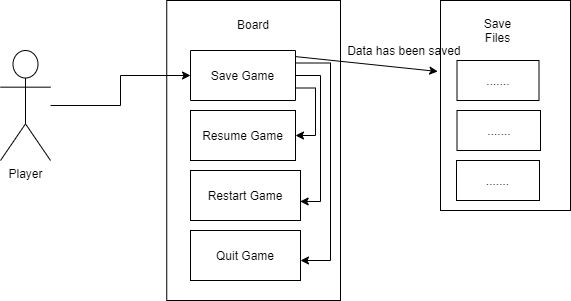
\includegraphics[scale=0.6]{images/SaveGame.png}
    \caption{Use Case Diagram - Save Game}
    \label{fig:SaveGame}
\end{figure}

\begin{center}
\setlength{\tabcolsep}{18pt}
\renewcommand{\arraystretch}{1.3}
\begin{tabular}{ |p{3cm}|p{10cm}| }
    \hline
    \rowcolor{green}
   Item & Description \\
    \hline
    Name & Save Game \\
    \hline
    Summary & The user is able to save the current progress \\
    \hline
    Actors & Player \\
    \hline
    Precondition & 
    \vspace*{-0.2in}
    \begin{enumerate}
        \item The player started the game
        \item The player pressed the save button
    \end{enumerate}  \\
    \hline
    Main Scenario &     
    \vspace*{-0.2in}
    \begin{enumerate}
        \item The player press the save button
        \item The current progress is saved in player's account
    \end{enumerate}  \\
    \hline
    Exceptions & \\
    \hline
    Postcondition &
    \vspace*{-0.2in}
    \begin{enumerate}
        \item Restart the game
        \item Resume the game
        \item Quit the game
    \end{enumerate}  \\
    \hline
    Priority & Medium \\
    \hline
    Traces to Test Cases & Added when test cases done  \\
    \hline
\end{tabular}
\end{center}

\newpage

%%%%%%%%%%%%%%%%%%%%%%%%%%%%% USE CASE 12 - View the best score

\subsubsection{Use Case 12 - View the best score} \label{uc:12}

\begin{figure}[htbp]
    \centering
    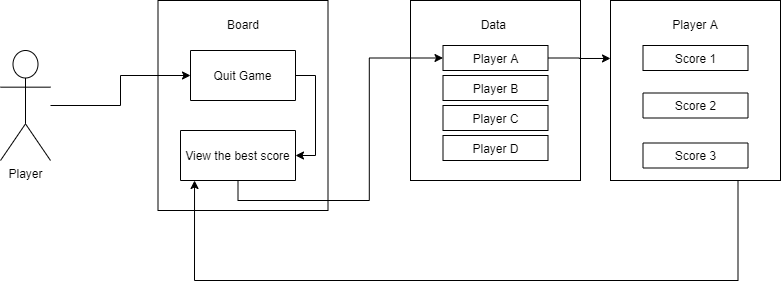
\includegraphics[scale=0.6]{images/ViewTheBestScore.png}
    \caption{Use Case Diagram - View the best score}
    \label{fig:ViewTheBestScore}
\end{figure}

\begin{center}
\setlength{\tabcolsep}{18pt}
\renewcommand{\arraystretch}{1.3}
\begin{tabular}{ |p{3cm}|p{10cm}| }
    \hline
    \rowcolor{green}
   Item & Description \\
    \hline
    Name & View the best score \\
    \hline
    Summary & A player can view the best score and scoreboard after the gameplay \\
    \hline
    Actors & Player \\
    \hline
    Precondition & 
    \vspace*{-0.2in}
    \begin{enumerate}
        \item The player finished the game
        \item The player pressed the view high score button
    \end{enumerate}  \\
    \hline
    Main Scenario &     
    \vspace*{-0.2in}
    \begin{enumerate}
        \item The player views the scoreboard which displays every gameplay scores and time
        \item The user views the best score
    \end{enumerate}  \\
    \hline
    Exceptions & \\
    \hline
    Postcondition &
    \vspace*{-0.2in}
    \begin{enumerate}
        \item Quit the game
    \end{enumerate}  \\
    \hline
    Priority & Low \\
    \hline
    Traces to Test Cases & Added when test cases done  \\
    \hline
\end{tabular}
\end{center}

\newpage

\subsection{Overview}

\section{Non-Functional Constraints}

In Kakuro, each puzzle consists of a blank grid with sum-clues in diverse location. The objective is to fill all empty squares using numbers from 1 to 9 so as the sum of each horizontal block equals the clue on its left, and the sum of each vertical block equals the clue on its top. Furthermore, no number may be used more than once in the same block.

One way to solve a Kakuro puzzle is incremental that is by using the current information on the board where you can find with certitude the value of a specific cell which can take only one possible value.

\section{User Interface}
\begin{figure}[htbp]
    \centering
    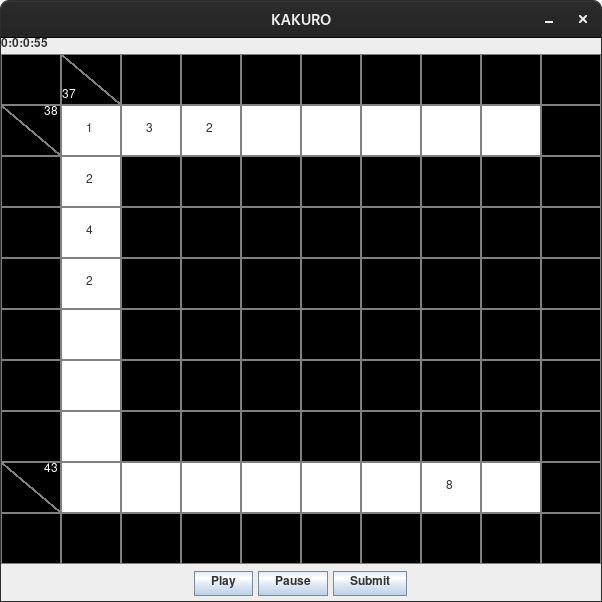
\includegraphics[scale=0.4]{images/UI1.png}
    \caption{Game Board}
    \label{fig:Game Board}
\end{figure}

In Kakuro, the User Interface should be concise and easy to navigate users to register,login,start and finish the game. It is the bridge connecting the users and our Kakuro game, a convenient and friendly user interface can guide the users through the whole game play in order to improve the users' overall experience. The user interface should help users to familiarize the game and guide them to complete the game successfully.

\begin{figure}[htbp]
    \centering
    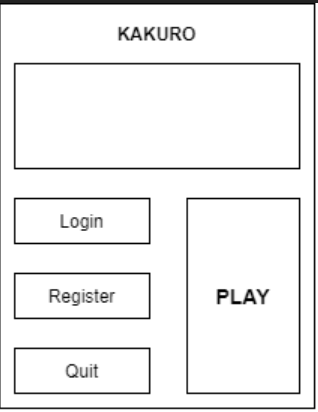
\includegraphics[scale=0.5]{images/UI2.png}
      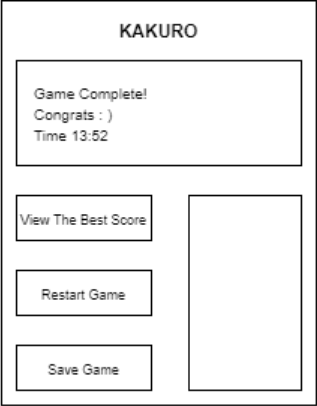
\includegraphics[scale=0.5]{images/UI3.png}
          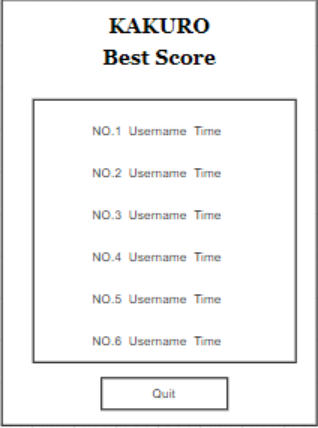
\includegraphics[scale=0.5]{images/UI4.png}
    \caption{User Interface}
    \label{fig:UI}
\end{figure}

\section{Design Constraints}
% MOCKED
"Lorem ipsum dolor sit amet, consectetur adipiscing elit, sed do eiusmod tempor incididunt ut labore et dolore magna aliqua. Ut enim ad minim veniam, quis nostrud exercitation ullamco laboris nisi ut aliquip ex ea commodo consequat. Duis aute irure dolor in reprehenderit in voluptate velit esse cillum dolore eu fugiat nulla pariatur. Excepteur sint occaecat cupidatat non proident, sunt in culpa qui officia deserunt mollit anim id est laborum."

\section{Glossary}



Grid/Game board\\\\
The grid will have a static size of 10x10, which consist of white and colored tiles. The white tiles consist of empty slots, where numbers are placed. On the other hand, the black tiles consists of numbers that are divided in a half cell. The black tiles fills the first row and first column entirely with its unique property that can be in half or full colored with appropriate numbers that acts as hints for the player.\\

High score\\\\
A high score consist of personal or overall scores of players based on how fast they completed the game.\\

Timer \\\\
A timer represents the number of times left to complete the game before losing the score.\\

Database\\\\
A data storage that runs on SQLite\\


\newpage

\section{References}

1) Introduction: https://en.wikipedia.org/wiki/Kakuro

2) Game Mechanics: https://www.kakuros.com/solve


\setlength{\parindent}{10ex}
\end{document}

